%!TEX TS-program = xelatex
%!TEX engine = xelatex

\documentclass{standalone}

\usepackage{fontspec}
\setmainfont{Fira Mono}
\usepackage{unicode-math}
\setmathfont[Scale=MatchUppercase]{STIX Two Math}
\setmathrm[Scale=MatchUppercase,
           BoldFont=STIX Two Text Bold]{STIX Two Math}
\setmathtt[Scale=MatchUppercase]{Fira Mono}

\usepackage{tikz}

\begin{document}
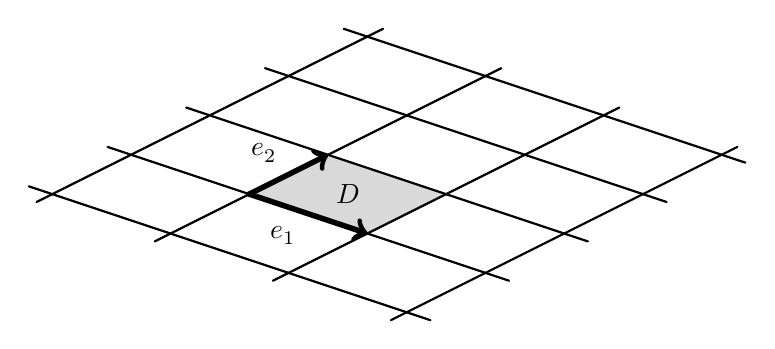
\begin{tikzpicture}[line cap=round,line join=round,x=0.5cm,y=0.5cm]
\fill[black!15] (0, 0) -- (3, -1) -- (5, 0) -- (2, 1) -- cycle;
\node at (2.5, 0) {$D$};

\draw [->,line width=2.pt] (0.,0.) -- (3.,-1.) node[midway, below left] {$e_1$};
\draw [->,line width=2.pt] (0.,0.) -- (2.,1.) node[midway, above left] {$e_2$};
\draw [line width=0.8pt] (-2.4,-1.2)-- (6.4,3.2);
\draw [line width=0.8pt] (-3.6,1.2)-- (6.6,-2.2);
\draw [line width=0.8pt] (-1.6,2.2)-- (8.6,-1.2);
\draw [line width=0.8pt] (0.4,3.2)-- (10.6,-0.2);
\draw [line width=0.8pt] (0.6,-2.2)-- (9.4,2.2);
\draw [line width=0.8pt] (3.6,-3.2)-- (12.4,1.2);
\draw [line width=0.8pt] (-5.4,-0.2)-- (3.4,4.2);
\draw [line width=0.8pt] (2.4,4.2)-- (12.6,0.8);
\draw [line width=0.8pt] (-5.6,0.2)-- (4.6,-3.2);
\end{tikzpicture}
\end{document}
